
\begin{figure}
  \centering
  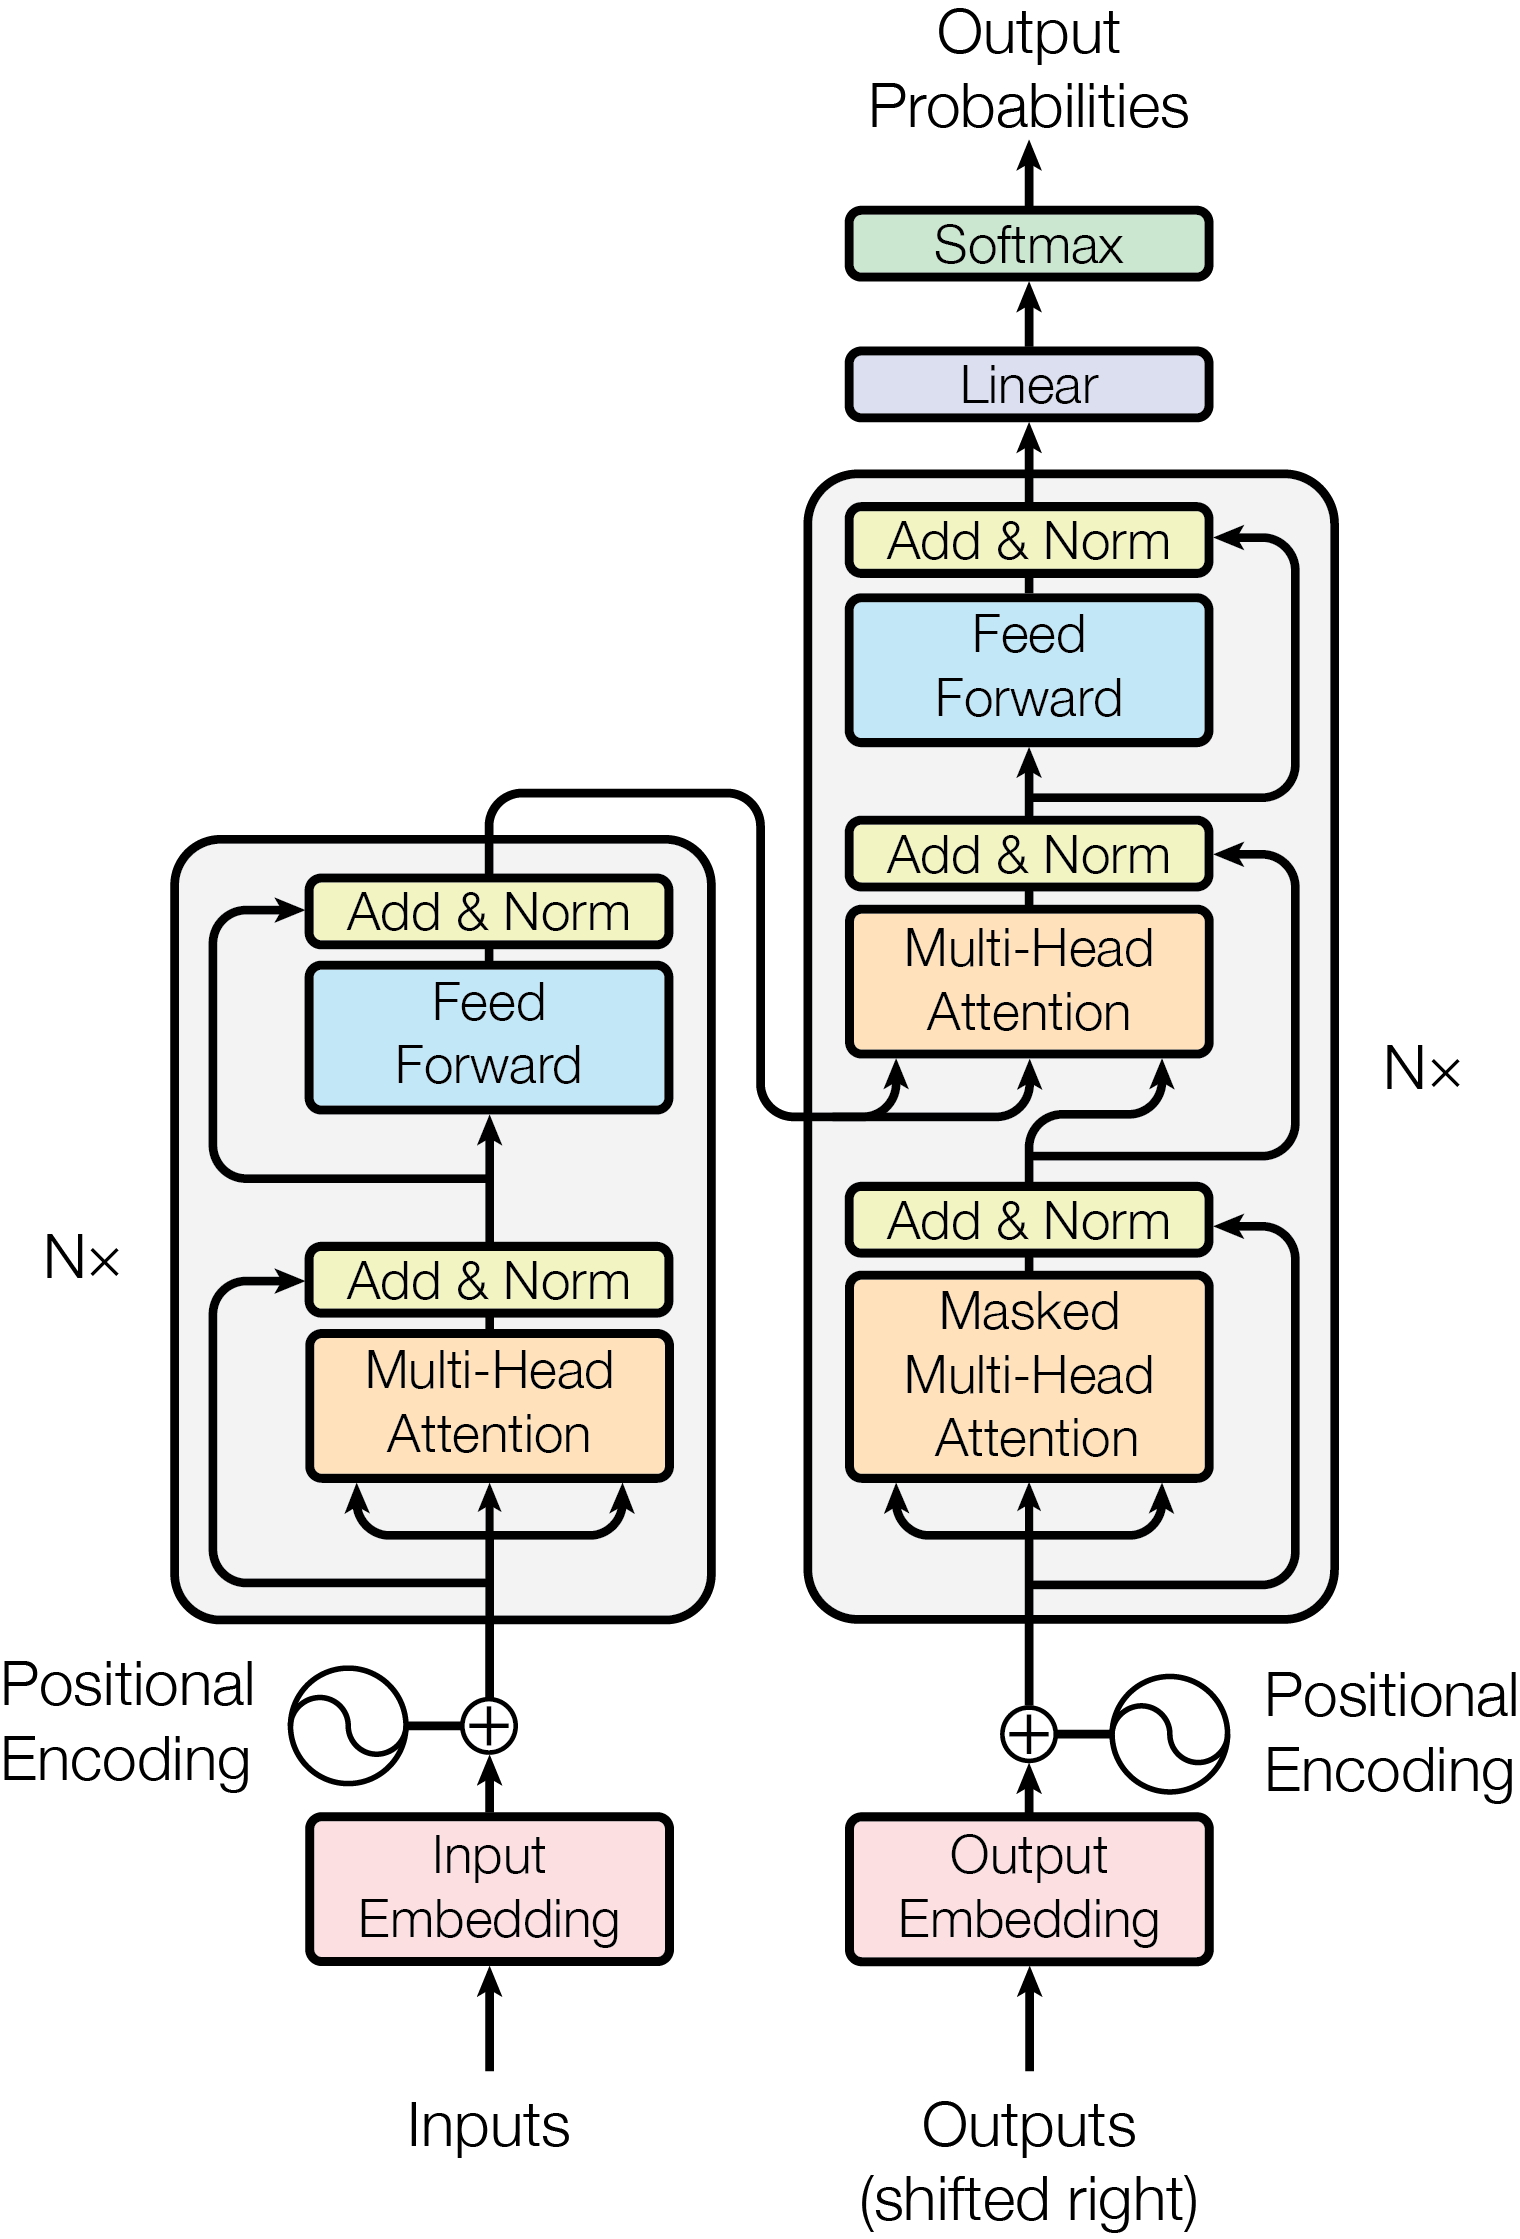
\includegraphics[scale=0.6]{Figures/ModalNet-21}
  \caption{Transformer - 模型架构。}
  \label{fig:model-arch}
\end{figure}

% Although the primary workhorse of our model is attention, 
%Our model maintains the encoder-decoder structure that is common to many so-called sequence-to-sequence models \citep{bahdanau2014neural,sutskever14}.  As in all such architectures, the encoder computes a representation of the input sequence, and the decoder consumes these representations along with the output tokens to autoregressively produce the output sequence.  Where, traditionally, the encoder and decoder contain stacks of recurrent or convolutional layers, our encoder and decoder stacks are composed of attention layers and position-wise feed-forward layers (Figure~\ref{fig:model-arch}).  The following sections describe the gross architecture and these particular components in detail.

大多数有竞争力的神经序列转导模型都采用编码器-解码器结构 \citep{cho2014learning,bahdanau2014neural,sutskever14}。这里，编码器将输入符号表征序列 $(x_1, ..., x_n)$ 映射到连续表征序列 $\mathbf{z} = (z_1, ..., z_n)$。给定 $\mathbf{z}$，解码器每次生成一个元素，逐个生成输出序列 $(y_1,...,y_m)$。在每一步中，模型是自回归的 \citep{graves2013generating}，在生成下一个元素时消费之前生成的符号作为附加输入。

Transformer 遵循这种总体架构，对编码器和解码器都使用堆叠的自注意力和逐点完全连接层，分别如图~\ref{fig:model-arch} 的左右两半所示。

\subsection{编码器和解码器堆栈}

\paragraph{编码器：}编码器由 $N=6$ 个相同层的堆栈组成。每层有两个子层。第一个是多头自注意力机制，第二个是简单的逐点完全连接前馈网络。我们在两个子层周围各采用一个残差连接 \citep{he2016deep}，随后是层归一化 \cite{layernorm2016}。也就是说，每个子层的输出是 $\mathrm{LayerNorm}(x + \mathrm{Sublayer}(x))$，其中 $\mathrm{Sublayer}(x)$ 是子层本身实现的函数。为了便于这些残差连接，模型中的所有子层以及嵌入层产生维度为 $\dmodel=512$ 的输出。

\paragraph{解码器：}解码器也由 $N=6$ 个相同层的堆栈组成。除了每个编码器层中的两个子层外，解码器插入第三个子层，该子层对编码器堆栈的输出执行多头注意力。类似于编码器，我们在每个子层周围各采用残差连接，随后是层归一化。我们还修改了解码器堆栈中的自注意力子层，以防止位置注意到后续位置。这种掩码，结合输出嵌入偏移一个位置的事实，确保位置 $i$ 的预测只能依赖于位置小于 $i$ 的已知输出。

% In our model (Figure~\ref{fig:model-arch}), the encoder and decoder are composed of stacks of alternating self-attention layers (for cross-positional communication) and position-wise feed-forward layers (for in-place computation).  In addition, the decoder stack contains encoder-decoder attention layers.  Since attention is agnostic to the distances between words, our model requires a "positional encoding" to be added to the encoder and decoder input. The following sections describe all of these components in detail.

\subsection{注意力} \label{sec:attention}
注意力函数可以描述为将查询和一组键值对映射到输出，其中查询、键、值和输出都是向量。输出被计算为值的加权和，其中分配给每个值的权重由查询与对应键的兼容性函数计算。

\subsubsection{缩放点积注意力} \label{sec:scaled-dot-prod}

% \begin{figure}
%   \centering
%   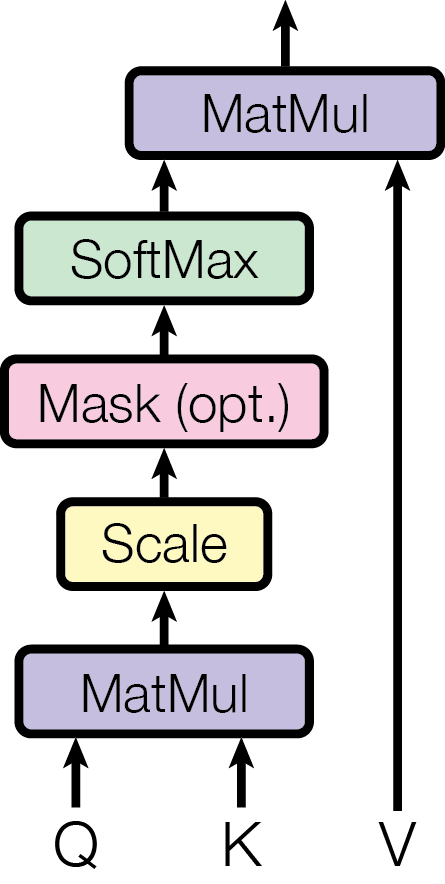
\includegraphics[scale=0.6]{Figures/ModalNet-19}
%   \caption{Scaled Dot-Product Attention.}
%   \label{fig:multi-head-att}
% \end{figure}

我们将我们的特定注意力称为"缩放点积注意力"（图~\ref{fig:multi-head-att}）。输入包括维度为 $d_k$ 的查询和键，以及维度为 $d_v$ 的值。我们计算查询与所有键的点积，将每个点积除以 $\sqrt{d_k}$，并应用 softmax 函数获得值的权重。

实际上，我们同时对一组查询计算注意力函数，将它们打包在矩阵 $Q$ 中。键和值也分别被打包在矩阵 $K$ 和 $V$ 中。我们计算输出矩阵为：

\begin{equation}
   \mathrm{Attention}(Q, K, V) = \mathrm{softmax}(\frac{QK^T}{\sqrt{d_k}})V
\end{equation}

两种最常用的注意力函数是加法注意力 \citep{bahdanau2014neural} 和点积（乘法）注意力。点积注意力与我们的算法相同，除了缩放因子 $\frac{1}{\sqrt{d_k}}$。加法注意力使用具有单个隐层的前馈网络计算兼容性函数。虽然两者在理论复杂性上相似，但点积注意力在实践中要快得多，空间效率也更高，因为它可以使用高度优化的矩阵乘法代码实现。 

%We scale the dot products by $1/\sqrt{d_k}$ to limit the magnitude of the dot products, which works well in practice. Otherwise, we found applying the softmax to often result in weights very close to 0 or 1, and hence minuscule gradients.

% Already described in the subsequent section
%When used as part of decoder self-attention, an optional mask function is applied just before the softmax to prevent positions from attending to subsequent positions.   This mask simply sets the logits corresponding to all illegal connections (those outside of the lower triangle) to $-\infty$.

%\paragraph{Comparison to Additive Attention: } We choose dot product attention over additive attention \citep{bahdanau2014neural} since it can be computed using highly optimized matrix multiplication code.  This optimization is particularly important to us, as we employ many attention layers in our model.

对于 $d_k$ 的较小值，两种机制表现相似，但对于较大的 $d_k$ 值，加法注意力优于无缩放的点积注意力 \citep{DBLP:journals/corr/BritzGLL17}。我们怀疑对于大的 $d_k$ 值，点积的大小增长很大，将 softmax 函数推入梯度极小的区域 \footnote{为说明为什么点积变大，假设 $q$ 和 $k$ 的分量是均值为 $0$ 方差为 $1$ 的独立随机变量。则其点积 $q \cdot k = \sum_{i=1}^{d_k} q_ik_i$ 的均值为 $0$ 方差为 $d_k$。}。为了抵消这个效果，我们将点积缩放 $\frac{1}{\sqrt{d_k}}$。


%We suspect this to be caused by the dot products growing too large in magnitude to result in useful gradients after applying the softmax function.  To counteract this, we scale the dot product by $1/\sqrt{d_k}$.


\subsubsection{多头注意力} \label{sec:multihead}

\begin{figure}
\begin{minipage}[t]{0.5\textwidth}
  \centering
  Scaled Dot-Product Attention \\
  \vspace{0.5cm}
  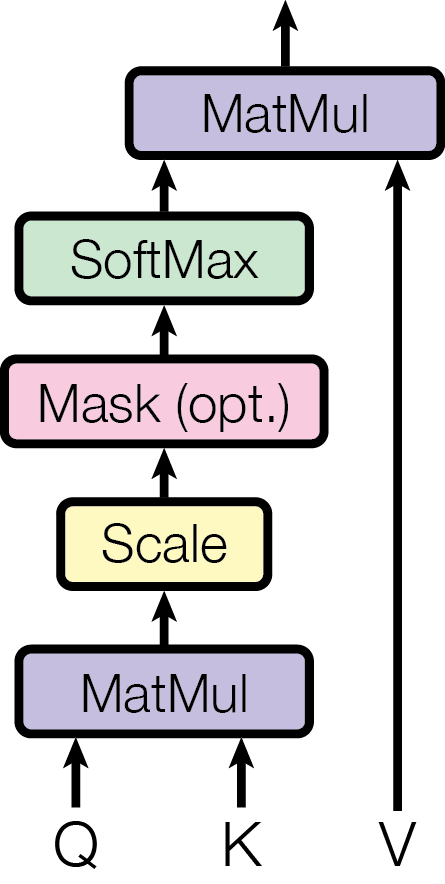
\includegraphics[scale=0.6]{Figures/ModalNet-19}
\end{minipage}
\begin{minipage}[t]{0.5\textwidth}
  \centering 
  Multi-Head Attention \\
  \vspace{0.1cm}
  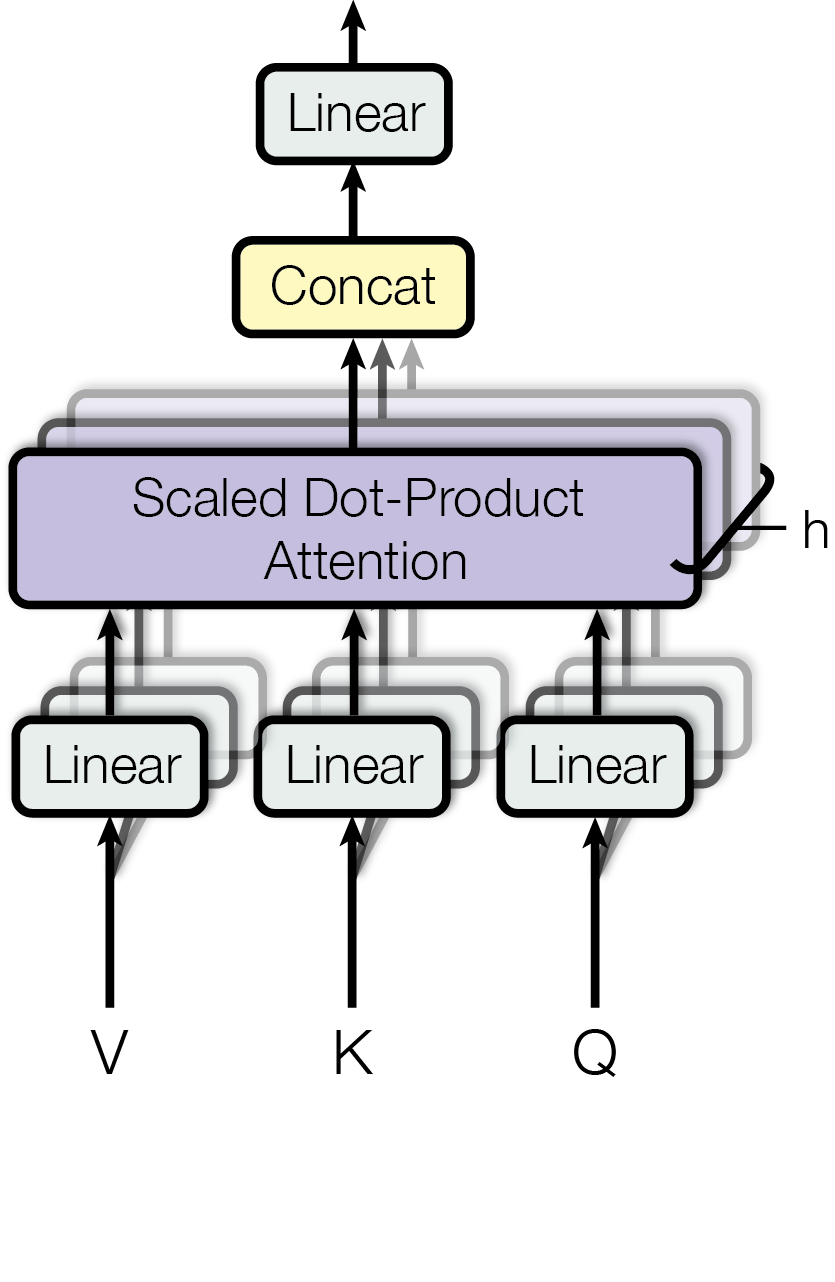
\includegraphics[scale=0.6]{Figures/ModalNet-20}  
\end{minipage}


  % \centering

  \caption{（左）缩放点积注意力。（右）多头注意力由并行运行的多个注意力层组成。}
  \label{fig:multi-head-att}
\end{figure}

与其进行单个注意力函数与 $\dmodel$ 维的键、值和查询，我们发现有益的是线性投影查询、键和值 $h$ 次，使用不同的学习线性投影到 $d_k$、$d_k$ 和 $d_v$ 维。
在这些投影的查询、键和值的每个版本上，我们然后并行执行注意力函数，产生 $d_v$ 维的输出值。这些被连接，然后再投影一次，产生最终的值，如图~\ref{fig:multi-head-att} 所示。

多头注意力允许模型同时关注来自不同位置的不同表征子空间的信息。使用单个注意力头，取平均会削弱这一点。

\begin{align*}
    \mathrm{MultiHead}(Q, K, V) &= \mathrm{Concat}(\mathrm{head_1}, ..., \mathrm{head_h})W^O\\
%    \mathrm{where} \mathrm{head_i} &= \mathrm{Attention}(QW_Q_i^{\dmodel \times d_q}, KW_K_i^{\dmodel \times d_k}, VW^V_i^{\dmodel \times d_v})\\
    \text{where}~\mathrm{head_i} &= \mathrm{Attention}(QW^Q_i, KW^K_i, VW^V_i)\\
\end{align*}

其中投影是参数矩阵 $W^Q_i \in \mathbb{R}^{\dmodel \times d_k}$、$W^K_i \in \mathbb{R}^{\dmodel \times d_k}$、$W^V_i \in \mathbb{R}^{\dmodel \times d_v}$ 和 $W^O \in \mathbb{R}^{hd_v \times \dmodel}$。


%find it better (and no more expensive) to have multiple parallel attention layers (each over the full set of positions) with proportionally lower-dimensional keys, values and queries.  We call this "Multi-Head Attention" (Figure~\ref{fig:multi-head-att}).  The keys, values, and queries for each of these parallel attention layers are computed by learned linear transformations of the inputs to the multi-head attention.  We use different linear transformations across different parallel attention layers.  The output of the parallel attention layers are concatenated, and then passed through a final learned linear transformation. 

在本工作中，我们采用 $h=8$ 个并行注意力层或头。对于每个，我们使用 $d_k=d_v=\dmodel/h=64$。
由于每个头的维度降低，总计算成本与具有完整维度的单头注意力相似。

\subsubsection{模型中注意力的应用}

Transformer 以三种不同的方式使用多头注意力：
\begin{itemize}
 \item 在"编码器-解码器注意力"层中，查询来自前一个解码器层，而记忆键和值来自编码器的输出。这允许解码器中的每个位置关注输入序列中的所有位置。这模仿了序列到序列模型（如 \citep{wu2016google, bahdanau2014neural,JonasFaceNet2017}）中的典型编码器-解码器注意力机制。

 \item 编码器包含自注意力层。在自注意力层中，所有的键、值和查询来自同一位置，在本例中是编码器中前一层的输出。编码器中的每个位置可以关注编码器前一层中的所有位置。

 \item 类似地，解码器中的自注意力层允许解码器中的每个位置关注解码器中到该位置为止的所有位置。我们需要防止解码器中的左向信息流以保持自回归属性。我们通过掩码（设为 $-\infty$）缩放点积注意力中对应非法连接的 softmax 输入中的所有值来实现这一点。参见图~\ref{fig:multi-head-att}。

\end{itemize}

\subsection{逐位置前馈网络}\label{sec:ffn}

除了注意力子层外，编码器和解码器中的每一层都包含一个完全连接的前馈网络，它被分别地且相同地应用于每个位置。这由两个线性变换组成，中间有一个 ReLU 激活。

\begin{equation}
   \mathrm{FFN}(x)=\max(0, xW_1 + b_1) W_2 + b_2
\end{equation}

虽然线性变换在不同位置相同，但它们在不同层之间使用不同的参数。另一种描述方法是两个核大小为 1 的卷积。输入和输出的维度是 $\dmodel=512$，内层的维度是 $d_{ff}=2048$。



%In the appendix, we describe how the position-wise feed-forward network can also be seen as a form of attention.

%from Jakob: The number of operations required for the model to relate signals from two arbitrary input or output positions grows in the distance between positions in input or output, linearly for ConvS2S and logarithmically for ByteNet, making it harder to learn dependencies between these positions \citep{hochreiter2001gradient}. In the transformer this is reduced to a constant number of operations, albeit at the cost of effective resolution caused by averaging attention-weighted positions, an effect we aim to counteract with multi-headed attention.


%Figure~\ref{fig:simple-att} presents a simple attention function, $A$, with a single head, that forms the basis of our multi-head attention. $A$ takes a query key vector $\kq$, matrices of memory keys $\km$ and memory values $\vm$ ,and produces a query value vector $\vq$ as 
%\begin{equation*} \label{eq:attention}
%    A(\kq, \km, \vm) = {\vm}^T (Softmax(\km \kq).
%\end{equation*}
%We linearly transform $\kq,\,\km$, and $\vm$ with learned matrices ${\Wkq \text{,} \, \Wkm}$, and ${\Wvm}$ before calling the attention function, and transform the output query with $\Wvq$ before handing it to the feed forward layer. Each attention layer has it's own set of transformation matrices, which are shared across all query positions. $A$ is applied in parallel for each query position, and is implemented very efficiently as a batch of matrix multiplies. The self-attention and encoder-decoder attention layers use $A$, but with different arguments. For example, in encdoder self-attention, queries in encoder layer $i$ attention to memories in encoder layer $i-1$. To ensure that decoder self-attention layers do not look at future words, we add $- \inf$ to the softmax logits in positions $j+1$ to query length for query position $l$.  

%In simple attention, the query value is a weighted combination of the memory values where the attention weights sum to one. Although this function performs well in practice, the constraint on attention weights can restrict the amount of information that flows from memories to queries because the query cannot focus on multiple memory positions at once, which might be desirable when translating long sequences. \marginpar{@usz, could you think of an example of this ?} We remedy this by maintaining multiple attention heads at each query position that attend to all memory positions in parallel, with a different set of parameters  per attention head $h$. 
%\marginpar{}

\subsection{嵌入和 Softmax}
类似于其他序列转导模型，我们使用学习的嵌入将输入标记和输出标记转换为维度 $\dmodel$ 的向量。我们也使用通常的学习线性变换和 softmax 函数将解码器输出转换为预测的下一个标记概率。在我们的模型中，我们在两个嵌入层和 pre-softmax 线性变换之间共享相同的权重矩阵，类似于 \citep{press2016using}。在嵌入层中，我们将这些权重乘以 $\sqrt{\dmodel}$。


\subsection{位置编码}
由于我们的模型不包含循环和卷积，为了使模型能够利用序列的顺序，我们必须注入关于序列中标记的相对或绝对位置的一些信息。为此，我们在编码器和解码器堆栈的底部向输入嵌入添加"位置编码"。位置编码具有与嵌入相同的维度 $\dmodel$，以便可以将两者相加。位置编码有许多选择，学习的和固定的 \citep{JonasFaceNet2017}。

在本工作中，我们使用不同频率的正弦和余弦函数：

\begin{align*}
    PE_{(pos,2i)} = sin(pos / 10000^{2i/\dmodel}) \\
    PE_{(pos,2i+1)} = cos(pos / 10000^{2i/\dmodel})
\end{align*}

其中 $pos$ 是位置，$i$ 是维度。也就是说，位置编码的每个维度对应一个正弦波。波长形成从 $2\pi$ 到 $10000 \cdot 2\pi$ 的几何级数。我们选择这个函数是因为我们假设它会允许模型容易地学习根据相对位置进行注意，因为对于任何固定的偏移 $k$，$PE_{pos+k}$ 可以表示为 $PE_{pos}$ 的线性函数。

我们也尝试了使用学习的位置嵌入替代 \citep{JonasFaceNet2017}，发现两个版本产生了几乎相同的结果（见表 \ref{tab:variations} 行 (E)）。我们选择了正弦版本，因为它可能允许模型外推到比训练中遇到的序列长度更长的序列长度。
